\documentclass[12pt,a4paper]{article}
\usepackage{times}
\usepackage{durhampaper}
\usepackage{harvard}
\usepackage{algorithm}
\usepackage{algpseudocode}
\usepackage{array}
\usepackage{graphicx}
\usepackage{subfig}
\graphicspath{ {images/}}


\citationmode{abbr}
\bibliographystyle{agsm}

\title{Investigation of Machine Learning Techniques for a Ball Balancing Task}
\author{Edward Hockedy}
\student{Edward Hockedy}
\supervisor{Dr. Magnus Bordewich}
\degree{MSc Computer Science}

\date{}

\begin{document}

\maketitle

\begin{abstract}
These instructions give you guidelines for preparing the design paper.  DO NOT change any settings, such as margins and font sizes.  Just use this as a template and modify the contents into your design paper.  Do not cite references in the abstract.

The abstract must be a Structured Abstract with the headings {\bf Context/Background}, {\bf Aims}, {\bf Method}, and {\bf Proposed Solution}.  This section should not be no longer than a page, and having no more than two or three sentences under each heading is advised.
\end{abstract}

\begin{keywords}
Put a few keywords here.
\end{keywords}

\section{Introduction}
\subsection{Background}
Robotics is a rapidly advancing field with a wide range of applications. The primary aim of a robot in most cases is to emulate and improve upon actions carried out by a human or enable the completion of a task a human is incapable of completing. Examples of such uses include job automation, social care, dangerous environment exploration, entertainment, and many more. One of the most difficult aspects of creating a working robot is programming how it will behave. In some specific cases it is sufficient to tell the robot exactly what it must do complete the task, and how to do it. In general, though, it is difficult to hard-code all actions a robot can take because there are many possibilites, and humans may not know how to describe the optimal behaviour. 

There are two methods studied here - supervised learning and reinforcement learning. Supervised learning provides examples of actions taken accross a range of states. From this, the robot learns which actions are good to take in each situation and can interpolate based on the learnt model what to do in an unseen state. This is equivalent to the robot observing a human complete the task. Reinforcement learning is the problem faced by an agent that must learn behaviour through trial-and-error interactions with a dynamic environment \cite{rl_survey}. The robot is told what a good state to be in is, and by trying out different actions the robot receives a reward or punishment dependent on the quality of the state it transitions to. Over repeated trials it updates its idea of what the optimal behaviour is to receive the most reward.

\subsection{Project Aim}
This project partly looks at different methods of enabling a robot to learn to complete the task of balancing a ball on a tray. The robot can observe the ball and carry out one of two actions, either tilt clockwise or anticlockwise, in an attempt to keep the ball in the centre and with a low velocity. 

The project also looks at the use of how a simulation of the ball and tray can be used for training. Both reinforcement learning and supervised learning require the robot to repeatedly trial or perform a task, which can be very time consuming to carry out on the actual robot. The simulation is not a perfect recreation of how the tray and ball behave in real life, so this project explores the suitability of using a simulation to approximate real world behaviour, and asses how well the learnt behaviour transfers from the simulation to the robot. 

The first stage of the project is to PRESENT/FUTURE TENSE? implement the maching learning techniques in simulation. Supervised learning data is created by a user controlling the simulation and behaviour is learnt with a neural network. For reinforcement learning the simulation takes actions by itself which are judged by a specified reward function. The learning algorithm is Q-learning, and behaviour is built up and stored in a Q-table. 

Once simulated behaviour is learnt it is moved to the robot and performance is assesed. Enhancements are the made based on the performance. Enhancements include making the simulation more accurately represent the robot, and experience replay. The final deliverables are the implementation of Q-learning to balance the ball on the real robot, and the implmentation of the neural network to balance the ball on the robot.


\section{Related Work}
Machine learning is widely used for teaching behaviour to robots. \cite{nao_balance} uses Q-learning to teach a Nao robot to balance in certain poses that it cannot make before learning. The state space is of size 9, with some states larger than others. The action space is of size $7^5$. This gives over 150,000 state-action pairs. The reward function is relatively simple - the robot receives a positive reward if it tays stable after making an action, proportional to how stable it is. It reveives a negative reward if it becomes unstable, with a large negative reward if it falls over. It was trained over 1000 episodes in simulation, where an episode was 100 movements, or until the robot fell. It was concluded that the robot successfully learnt to blance in the poses. Reinforcement learning is commonly used in the form of a deep Q-network, as in \cite{sim_robot_arm} and \cite{robot_wheel}. 

Supervised learning is not commonly used in sophisticated robot behaviour learning. \cite{nn_then_dnn} uses a neural network trained in a supervised maner to create an initial reward approximation before performing reinforcement learning with a deep neural netwok. It was concluded that the pre-training helped the reinforcement learning converge faster. The tasks tested were the mountain-car problem, and a simulated autonomous wheeled robot.

Simulating the robot to decrease training times is common in literature. \cite{sim_robot_arm} investigates the task to grab a cube with a robotic arm after training in a simulation. The simulation closely models the robot arm. When the learnt behaviour was transferred to the real arm, the behaviour was closely followed until the point where the hand should have grabbed the cube, showing a not quite perfect behaviour recreation from simulation to real world despite a detailed simulation. \cite{arm_sim_door} also studied a robot arm, again with a sophisticated simulation. The tasks studied include reaching a random target, pulling a door, and moving an object. Discount factor was 0.98 and learn rate was a low value of 0.001 or 0.0001. Results show success when moving behaviour to the real world, but in some cases it required a lot of training. \cite{nao_football} uses reinforcement learning to train a Nao robot to kick a football. The training takes place in a simulation package capable of simulating the behaviour of the entire robot, thus modelling the real world very closely. 

Experience replay is used commonly, as in \cite{air_hockey} where it is used to speed up training. This is necessary because the task of learning to score with an air hockey puck requires lots of trials and a simulator was not used. Another interesting point about this paper is its assumption that the best action to take is always hitting the puck at maximum speed. This is a reasonable assumption, but brings up the question of the impact of making assumptions. It reduces the action-state space, but could cause issues if the assumption is an incorrect one. Experience replay is successfully used by \cite{er} in conjunction with Q-learning for the tasks of keeping an inverted pendulum up, moving a robot arm, and a robot goal keeper. There are all tasks of a similar complexity to the ball balancing task. The paper concludes that experience replay performed well in simulation and real-world, and outperformed Q-learning. Experience replay is also addressed by \cite{er_deeper}. It highlights the fact that the amount of experience replay data can have a detrimental effect on performance, and that size of experience replay buffer should be chosen carefully even for simple tasks.  


\section{Design}

\subsection{The Task}
The task chosen for the robot to learn to perform was to balance a ball on a tray. The ball can move either to the left or the right. The goal for the robot is to keep the ball stable - in the middle of the tray with the velocity low. This is done by performing one of a number of three actions, tilt the tray clockwise, tilt the tray anticlockwise, or keep the tray at the angle it currently is. At each step of the task the robot can observe information about the environment. This information comprises of the horizontal position of the ball relative to the robot, with the origin at the centre, the horizontal velocity of the ball, and the angle the tray is currently tilted at. These pieces of information are continuous and must be mapped to discrete states. For example, the position of the ball is grouped into one of 10 possible positions on the tray. The combination position, velocity and angle, makes up the current state of the environment. The task is to have the robot learn what the best action to take given any state.

This task was chosen because it seemed simple enough to be achievable by a robot with the chosen learning techniques. The number of states is fairly small, but big enough that it is hard to outright describe what to do in every scenario. It is also complex enough to be difficult to describe without mathematically modelling the whole system, but simple enough that the leant model can interpolate to unseen scenarios. The task is also one achievable by humans in a basic sense of just standing still, but becomes difficult when extra tasks are included such as walking forward. As such it is hoped that the robot could surpass human performance if it learns well enough. The task has obvious real world applications. Whilst the level of performance achieved in this project is insufficient to have much real world impact, a high level implementation of this behaviour could be used to carry object accross a room, perhaps to an immobile patient, or to carry a person out of a dangerous environment.

\subsection{The Robot}
The robot used is the humanoid Nao from SoftBank robotics. It is fully programmable using the Python API and allows for full control over the angles and position of joints. It has built in vision capabilities from the cameras located on its head. For the setup of this task, the Nao robot is standing with its arms stretched out. It grabs on to a cardboard tray and holds it flat in front of it. There is a small track that the ball sits in to prevent it from falling off the back or front of the tray, and two side buffers to prevent it from falling off the sides. The robot has built in functionality to track a red ball which is the method used in this project. At any time the position in 3D space of the ball can be calculated by the robot. The velocity can then be obtained by observing the change in position over a given time period. The tray is tilted by the robot moving it arms. To determine the range of possible angles the robot can move between, the robot's arms were positioned by hand and the angles of the upper body joints were recorded. They were then manipulated so that the same angle could be recreate but in the opposite direction. The robot can then interpolate any angle between the maximum and minimum by taking a proportion of the maximum tilt and minimum tilt and adding the angles together.

INSERT PHOTO OF ROBOT AND TRAY

\subsection{Simulation}
The simulated environment is two-dimensional and comprises of a ball that rests on a tray that can tilt. The tray has barriers at either end to stop the ball from rolling off the ends of the tray. The tray can be tilted up to a maximum angle in each direction. This simulation was built using the Pymunk physics engine. At each stage of the simulation the position and velocity of the ball can be directly read, as well as the angle of the tray.  

\subsection{Reinforcement Learning Approach}
The agent (the robot/simulation) learns how to balance the ball by trying different actions whilst aiming to get the ball into a good state. The method of reinforcement learning used in this project is Q-learning. Q-learning is a model-free reinforcement learning technique. Being model-free means there is no pre-learnt model that the actions are based off, it relies fully on the trial-and-error experiences for learning actions. Over time, the agent learns the best action to take for each state. This information is stored in a Q-matrix, a large matrix with a cell for each possible state the ball can be in. For each cell there is an array of length equal to the number of possible actions the agent can take. A value is stored for each action, with the value representing how good of an action it is given the current state. Learning starts with the agent observing the state it is in. It then looks at the Q-matrix and decides what the best action it can take is - the one with the greatest value. There is a probability that a different action will be taken instead - this allows for trialling different actions that may end up being more beneficial. It carries out the action and observes the state it ends up in. It also receives a reward dependent on how good this new state is. The value for the action taken from the old state is then updated using the exising value, the reward, and the value of the best possible action to take given the new state. The intuition behind using the best value of the new state is that Q-learning assumes the agent is follwing an optimal policy - the best possible chain of transitions between states, taking the optimal action each time. This is of course not the case during training, but over time it should converge to this. The update policy can be formalised as:
\[Q(s_t, a_t) = (1 - \alpha) \cdot Q(s_t, a_t) + \alpha\cdot(r_t + \gamma\cdot max Q(s_{t+1}, a)) \]
$s_t$ is the state at time t \\
$a_t$ is the action taken at time t \\
$r_t$ is the reward observed by taking $a_t$ from $s_t$\\
$\alpha$ is the learn rate. The higher this is the higher the updated value takes into account the reward and future state information compared with the existing value\\
$\gamma$ is the discount factor. The higher this is, the more important future values are taken to be. A small value only looks at the immediate future of the next few transitions\\

For the implementation of Q-learning in this project, the reward was determined in two ways. The first was with a very specific reward, based on what a human would intuitively think is the best action to take at each step. It used both the current state information and previous state information. The reward is decided based on the criteria outlined in algorithm \ref{ql_specific}.
\begin{algorithm}[H]
	\caption{Calculate reward using very specific criteria}
	\label{ql_specific}
	\begin{algorithmic}[1]
		\State $reward = 0$
		\If {$current\_velocity > 0$ \textbf{AND} $current\_angle > previous\_angle$}
			\State $reward = 1 - |\frac{current\_position}{tray\_width}|$
		\ElsIf {$current\_velocity < 0$ \textbf{AND} $current\_angle < previous\_angle$}
			\State $reward = 1 - |\frac{current\_position}{tray\_width}|$
		\ElsIf {$|current\_velocity| < max\_velocity*0.01$ \textbf{AND} $|current\_position| < |previous\_position|$}
			\State $reward = 1 - |\frac{current\_position}{tray\_width}|$
		\Else 
			\State $reward = -1 * (1 -|\frac{current\_position}{tray\_width}|)$
		\EndIf
	\end{algorithmic}
\end{algorithm}
Algorithm \ref{ql_specific} gives a positive reward if the ball has a positive velocity (left to right) and the tray has moved anticlockwise, effectively slowing it down, and vice-versa on line 4. It also gives a positive reward if the ball is at the very low speed of 1\% of the maximum speed, and moving towards the centre of the tray. Since the tray is centred on 0, the magnitude of the position determines how close to the centre the ball is, with a smaller magnitude meaning the ball is closer. If none of these cases are matched, then a negative reward is given. In each case of the reward, the size is determined by how far the ball is to the centre, with a bigger reward being given if the ball is closer to the centre.

The second reward scheme is much simpler, using only the current state information to specify the states that deserve a good reward, with everything else getting a negative reward. The reward scheme is outlines in algorithm \ref{ql_general}.

\begin{algorithm}[H]
	\caption{Calculate reward using very general criteria}
	\label{ql_general}
	\begin{algorithmic}[1]
		\State $reward = 0$
		\State$pos\_range$ = length of tray * 0.2
		\State$vel\_range$ = maximum velocity * 0.2
		\If {$- pos\_range< pos < pos\_range$
			\textbf{AND}
			 $-vel\_range < vel < vel\_range$}
			\State $reward = 1$
		\Else 
			\State $reward = -1$
		\EndIf
	\end{algorithmic}
\end{algorithm}
Algorithm \ref{ql_general} gives a positive reward if the ball is in one of the segments determined to be good. The $pos\_range$ and $vel\_range$ variables determine the range of ball positions and velocities that are considered good. Maximum velocity is the maximum velocity the ball can reach by letting it roll from one end to the other at maximum angle.

The training begins with the ball dropped into a random position and the tray at a random angle. At each step the agent chooses the action it thinks is the best for the given state. No prior knowledge is given for Q-learning, so all table values are 0. In order to assign values, at the start there is a very high probability of taking a random action. This probability is known as the explore rate. This allows the agent to slowly build up some scores for taking actions at different states. Over time the Q-matrix fills up and the values should start to converge. The explore rate decreases over time to allow the agent to start taking the best actions. Most states will have been sampled after enough time, so exploration is not needed. The Q-matrix should end up with the states all suitably sampled, and the rewards/punishments should have propagated through via the update function such that a distribution of state quality exists through the matrix. 
\subsection{Supervised Learning Approach}
The first step in the supervised learning approach was to generate the training data. To do this the simulation was altered so that it could be moved by user input. A ball would be dropped onto the tray at a random angle, and a user could press keys to turn the tray one angle segment clockwise or anticlockwise, depending on what was required to keep the ball balanced. At each key press, the state and action taken was recorded. This was repeated over many iterations to build up a reasonably sized data set that covered many situations. About 360 items of training data were recorded.The model used to learn the pattern is a neural network.
%A neural network is a way to theoretically simulate any function, by combining many simple, linearly-separable functions known as neurons. The neurons e
%exist in layers with one input layer and one output layer. Between the layers exists weights from each neuron to each neuron in the next layer. The network is trained by passing through the input data. Each neuron receives some input from the previous layer, maps the combination of input values to an output value depending on its function, then outputs a value that goes to the next layer. Once the input data has passed through the network, the output from the network is compared with the actual output from the training data. The difference is calculated and that error is used to refine the weights between the neurons. As more data is passed through, the network gets refined and begins to learn which inputs lead to which outputs.

For this project, then input value is the state of position segment, velocity segment and angle segment. The output is one of the three possible actions - tilt left, tilt right, or don't tilt, encoded with one-hot encoding. 


\subsection{From Simulation To Robot}
Once trained, the Q-matrix and neural network could both be used in conjunction with the robot. With the tray held out and the ball place on, the robot will track the ball and take actions based on what the neural network or Q-matrix decides is best. There were a few difficulties that arose with using the robot, as well as some parameters that needed to be chosen. The biggest issue was that the arms of the robot overheated quickly. For safety reasons, this means the stiffness in the overheated joint goes to zero meaning the joint cannot be moved. This usually happened about ten minutes after having the robot move its arms frequently. This was not a huge issue in the long run because the focus was to do all training in simulation, but any training or data collection that happened on the robot because difficult and time consuming when waiting for the robot to cool down. To circumvent this, two robots were used so one could cool down whilst the other was used. This issue very much highlights the usefulness of simulation in robot movement training.

Another issue was the accuracy of the ball tracking. The built in tracker could detect the position at any point by continuously calling the track function in a thread running in the background. Frequency of update caused issues. A more frequent update meant the changes in position were small, so the relative error in position detection was greater. Too infrequent updates limited the number of actions the robot could take.
% An issue arose when choosing the frequency of updating the ball information however. Too frequent updates meant the values may not update, and as such the velocity value would be zero which is often not the case. Too infrequent updates could mean that the robot is limited in the number of actions it can perform, since there must be a change in state otherwise an action is taken twice in a row. Since actions are limited by ball readings, if there are too few it means there may not be enough actions take in order for the tray to move the required amount to keep the ball balanced. Since the tray must move through the states one by one, if the updates are too slow then the ball may have moved past before any meaningful movement can occur. The accuracy of the method as a whole is also not perfect, and position value can vary quite a bit even for cases where the ball does not change position. Less frequent updates mean the error has less impact, but again less frequent updates can lead to issues.

The change of angle function calls to the robot joints are non-blocking. This means that as soon as an update to a joint is called, another one can be made. As such, it can limit the robot's ability to quickly switch between two angles, something that occurs quite often when balancing. Instead, the robot will stick to a single angle - problematic if that angle is not flat but the tray was supposed to fluctuate between angles either side of that flat angle. 

\subsection{Refining Simulation}
In the case of the reinforcement learning, the robot did not successfully emulate the simulation to the desired quality. The behaviour mainly consisted of the ball rolling to one end, the robot tilting the tray from the extreme of one angle to the other extreme, and the ball rolling to the other end. From observing this behaviour it was seen that there are only about 5 actions taken from the ball travelling from one end of the tray to the other. More actions were required to fully rotate the tray to a meaningful angle, and so the current state of the Q-matrix was not sufficient. In particular, if the robot took an action that was not optimal because the Q-matrix was insufficiently trained, then it could completely ruin the robots ball balancing ability. There are quite a few states where the difference in value for each action was minimal, since they were far from an optimal state and each action gave the same reward. The only disparity came from which action was taken most recently, as this will have had the most recent value update. 

To help with the non-optimal action being chosen, a "Q-matrix consensus" was taken when choosing an action. This takes into account the best action for the current state, but also the best actions for the states with a velocity segment difference of one either side, and the states with a position segment different either side. Assuming the current state does not involve the maximum or minimum velocity or position, this gives five votes for what the best action to take is. The action with the highest number of votes is taken. In the result of a tie, the original action is taken. The intuition behind this is that the states considered are similar to the current state, so will most likely have similar optimal actions. So in the case that the current state's values have not converged in the Q-matrix, it is hoped that some of the others have, leading to a better estimation of what the optimal state is. 

After seeing how the simulated behaviour worked with the robot, the simulation was changed to reflect the robots mechanics more closely with the hope of learning to deal with the difficulties present in the robot. The two behaviours incorporated into the robot are the delay between actions, and the overall speed of the ball. The delay between actions helps model the speed of the robot updating of the tray angle, which is slower then the simulation. After the tray has moved, it waits a set number of frames before deciding on the new action to perform. The speed of the ball is reflected in the simulation by increasing the number of steps taken per frame of the simulation. 

After training in the simulation for the same number of iterations of the original simulation, performance was definitely worse. However, this was not unexpected. Unfortunately, performance on the robot showed little improvement. 

\subsection{Experience Replay}
Experience replay is when data acquired during the online-learning process are stored and presented repeatedly to the underlying RL algorithm \cite{er}. A dataset of many actions taken by the robot was recorded. By running through this data and updating it with the Q-learning algorithm, it is hoped that the optimal behaviour is learnt using robots own actions instead of simulated actions. This means the actions are the most accurate representation of what the robot would actually do. The data stored comprises of an initial state, the action taken by the robot (not necessarily the one it believes to be optimal), the state it ends up in, and the reward received. Experience replay uses a Q-matrix trained in simulation as the Q-matrix  for the update function. To train in this way, an experience is randomly chosen. The pre-learnt Q-matrix is then updated for that state and action using the recorded reward and the future state value taken from the pre-trained Q-matrix for the state achieved by the robot. When collecting the data, to allow for a wide range of actions to be recorded, the robot was set to try to balance the ball as normal, but with a high possibility of performing a random action. Over time, this built up a dataset of many actions taken from many states. The new state reached for an action from a given state can vary a lot for the robot, so multiple readings could be stored for each state. The hope of this was to repeat the robot's actions many times without the robot so that it could learn which of those actions are beneficial. Since the robot doesn't actually have the ability to train on itself in real life, it cannot test which of its actions work well. There may be a large number of actions that are beneficial for states in the simulation, but not for states in the real robot, and vice-versa. 

Unfortunately, once again the improvement was not significant, but perhaps marginally better. The most interesting observation was that the simulation, when ran after experience replay, mimicked the behaviour of the robot quite closely - the ball was rolled from end to end. This shows that the simulation was capable of learning the robot's behaviour, but not the other way around. MOVE TO RESULTS?

\section{Results}
The success of a learnt behaviour for this task cannot be fully quantified as there is no end state. Instead the performance over time can be observed and used as a way to assess how well the learnt behaviour performs. If after training the ball is moving from side to side then it is clearly not balanced well. If it stays in the middle, it has successfully been balanced. For each training run, the position at each step of the simulation was recorded. This information can be plotted on a graph showing the motion of the ball over time, and is the metric used here to assess performance of each method. 

The results presented here show the performance of each method at each stage of its development. This includes training in the simulation and performance on the robot. They may also show refinement of parameters, or any optimisations made to get to the apparent best performance of the method. 

\subsection{Q-learning Parameter Refinement}
The first stage in achieving the best performance from the Q-learning was to find the best parameters that made the Q-matrix converge fastest.
\begin{table}[htb]
\centering
\caption{Q-learning parameters}
\vspace*{6pt}
\label{q_params}
\begin{tabular}{>{\raggedright}p{0.2\linewidth}p{0.55\linewidth}p{0.17\linewidth}}\hline
Parameter & Description& Tested Values\\ \hline\hline
Initial exploration rate & The starting probability of taking a different action to the one though to be the optimal & 0.2, 0.5, 1\\ \hline
Exploration rate reduction frequency & The number of times the exploration rate is reduced & 5, 10, 20\\ \hline
Exploration rate reduction value & The percentage to reduce the exploration rate by & 10, 20, 33.3, 50 \\\hline
Learn rate & The proportion the updated value in the Q-matrix is made up from learnt information compared to existing information & 0.1, 0.4, 0.5,  0.7 \\\hline
Discount factor & The influence future rewards have on updating the value for the current state and action & 0.5, 0.8, 0.9, 0.99 \\\hline
\end{tabular}
\end{table}
To refine these values, a grid search was performed to find the best combination. It is likely that many of these parameter values are dependent on each other, so it was important to test all combinations of different values.

Each of the following tests were ran for 50000 iterations, with an iteration consisting of seeing the current state, picking an action, and performing the action.

The parameters that concern the exploration rate are not independent, so all possible combinations of their values were tested. The quality of each parameter combination was judged by analysing the position of the ball over 5000 time frames once trained, and with explore rate set to 0. The best parameter combination was the one that gave the graph with the ball closest to 0 for the longest amount of time, and fewest movements to the edge of the tray. The best combination of parameters was found to be initial exploration rate = 0.5, exploration rate reduction frequency = 20, and exploration rate value = 1.5. An initial exploration rate of 0.5 makes sense, since at the start there is no optimal action for any state - each action has an initial value of 0, so the first action is chosen by default. Having an exploration rate of 0.5 means half the time that action will be taken, and the other half of the time the other action will be taken making it completely random. This is a good way to get a good starting sample of actions throughout the matrix. The combination of reduction value multiplier 1.5 and reduction frequency 20 has no direct explanation, it just seems to be the case that that speed and rate of phasing out the exploration rate works well. It allows for sufficient exploration whilst training but diminishes quick enough to not cause random actions when the best actions have already been found. Figure \ref{f1} shows the performance of the trained Q-matrix with these parameters over the 5000 time frames.

\begin{figure}[H]
	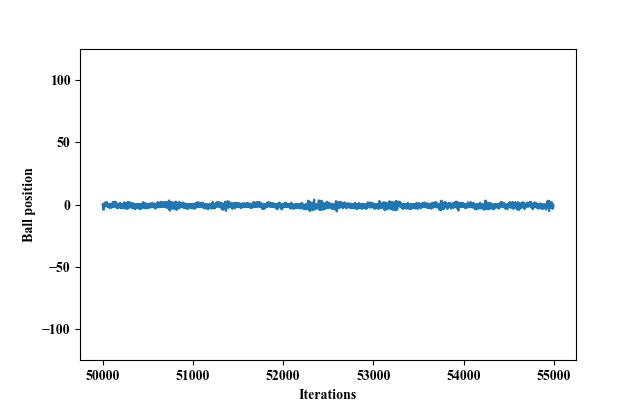
\includegraphics{100_small}
	\caption{The position of the ball over 5000 actions. Note that the width of the tray is 125 in each direction, so the ball stays very confortably in the centre}
	\label{f1}
\end{figure}
\begin{figure}[H]
	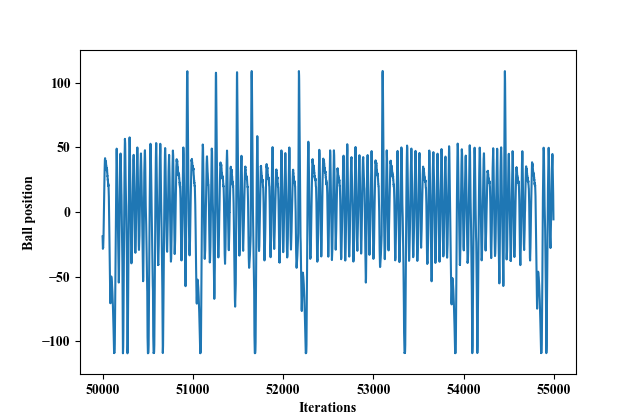
\includegraphics{101_small}
	\caption{An example of learnt behaviour that was not successful. The initial eploration rate was 0.2, reduction value was 1.5, number of reductions was 5. The repetition of the pattern shows that it has slightly learnt the ability to balance, however the amplitude is large. The ball also goes to the end quite frequently}
	\label{f2}
\end{figure}
%Sims 88 to 115 compares exploration rate stuff
% After 1st round of tests, 100 was best. This is erv:1.5, init:0.5, num:20. About 30000 iterations to converge
%\subsubsection{Initial exploration rate}

For learn rate and discount factor, low values of both gave poor results, and for the higher values, difference in performance was relatively small. However, through repreated tests it was found that the best values were a learn rate of 0.4 and a discount factor of 0.9. These results make sense. The learn rate is just below half, showing that the new information is important to the updating process, but is just a bit less important than the existing data. Anything higher could drown out the existing value stored, and since there is quite a lot of exploration, especially early on, it is important to not let the agent change its values too hastily. The discount factor is high since for a task like this because future actions are important. If not, it would send the ball to the centre of the tray as quick as possible, whether sometimes it is better to move it gradually to avoid overshooting. A possible reason 0.9 was superior to 0.99 (if only marginally) is that it is sometimes important to focus on the very short term, for instance when right at the edge of the tray - it is better to move the ball away quickly than roll off.

Convergence speed is another important aspect to learning. In a small task like this training takes less than a minute. For a larger task however, it is important to reach the desired performance level as soon as possible. It is hard to know when the task is fully leant since there is no exact completion criteria. However, looking at the plot of position against time for the whole learning procedure can show when the ball is kept in a constant position. Figure \ref{f3} shows this for the agent learning over 50000 iterations with the refined parameters.
\begin{figure}[H]
	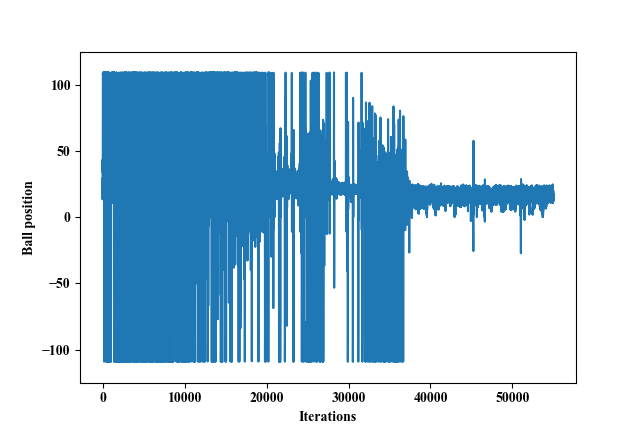
\includegraphics{153_small}
	\caption{The position of the ball over an entire training session. At the start the ball rapidly rolls between either side of the tray. Over time this becomes less frequent as behaviour to prevent this is learnt, and the random actions happen less frequently. By the end of the training, the ball is kept consistently in the middle of the tray.}
	\label{f3}
\end{figure}
Figure \ref{f3} shows that convergence happens at about 30000 time steps. It is not sufficient to cut off training at 30000 iterations however. Since exploration rate is linked to the number of iterations, with the same initial parameters the learning would be different. Also, it is probably best to continue learnig to solidify behaviour. 

Table \ref{q_params} shows the final values that gave the best performance for Q-learning out of the ones trialled. They may not be the optimal, but testing suggests they will be very close, and any improvemnts will be minro. The focus of the project is not to find the absolute best parameters for the task, so these values will suffice as they give a suitable Q-matrix convergence speed.
\begin{table}[htb]
\centering
\caption{Final Q-learning parameters}

\label{q_params}
\begin{tabular}{>{\raggedright}p{0.4\linewidth}p{0.2\linewidth}}\hline
Parameter & Refined Value\\ \hline\hline
Initial exploration rate & 0.5\\ \hline
Exploration rate reduction frequency & 20\\ \hline
Exploration rate reduction value & 33.3\% \\\hline
Learn rate & 0.4 \\\hline
Discount factor & 0.9 \\\hline
\end{tabular}
\end{table}


\subsection{General Reward vs Specific Reward for Q-learning in Simulation}
\begin{figure}[H]
	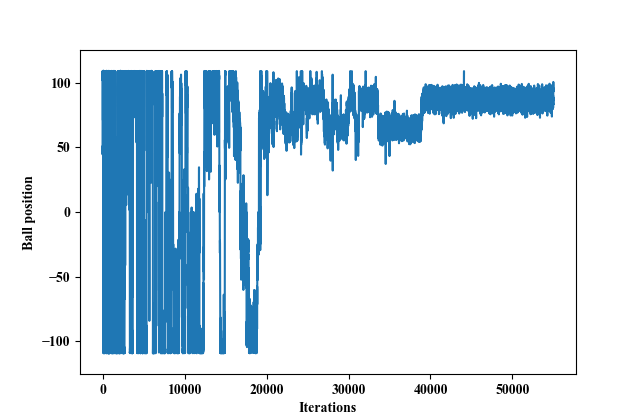
\includegraphics{157}
	\caption{The position of the ball when training with a detailed reward function.}
	\label{f5}
\end{figure}
For the parameter tuning, the reward used was the general reward. Figure \ref{f5} shows the performance of the trainer as it learns with the specific reward function over 50000 iterations. It appears to converge faster than the more general reward - convergence happens after about 20000 steps. However, the position on the tray that it keeps the ball is quite off centre. This can be considered balanced, but to give it maximum chance to keep balanced in the case of sudden movement, a central position is preferred. A specific reward likely gives this result as it is focussed on bringing the ball to a stop as soon as possible, and works to counteract any movement that may accelerate the ball. As such, it gets stuck wherever it is and never allows the ball to accelerate even a small amount to the centre of the tray since there is no consideration of future actions. TALK ABOUT THE BIT TO RE CENTRE IT

\subsection{Neural Network in Simulation}
To find the best neural network with the shortest training time, the parameters shown in table \ref{nn_params} were tested. The struture format is given as the number of neurons for each layer, so (x, y) has x neurons in the first layer and y neurons in the second layer. Th number of epochs is the number of times the trainer goes through the entire data set. Results showed that all combinations except for the (2) structure (single layer with two neurons) and 50 training epochs worked sufficiently. By comparing the graphs of the ball position over time for the trained network, as well as the time to train, the best structure was decided to be (2, 2). Other structures worked similarly well but the smaller structure meant shorter training time and less chance of overfitting. The number of epochs chosen to be best was 100 as it was enough to train sufficiently, did not take too long, and is less likely to cause overfitting compared to the larger number of epochs. Figure \ref{nn_param_test} shows the position over time for the trained network of chosen size. It balances the ball very well.
%from about 60 to 92 are the tests for nn params
\begin{table}[htb]
\centering
\caption{Neural network parameters. The best structure was (2, 2), best number of epochs was 100.}
\label{nn_params}
\begin{tabular}{>{\raggedright}p{0.3\linewidth}p{0.4\linewidth}}\hline
Parameter & Tested values\\ \hline\hline
Hidden layers structure & (2), (5), (10), (2, 2), (5, 5), (10, 10)\\ \hline
Number of training epochs & 50, 100, 150, 200\\ \hline
\end{tabular}
\end{table}

\begin{figure}[H]
	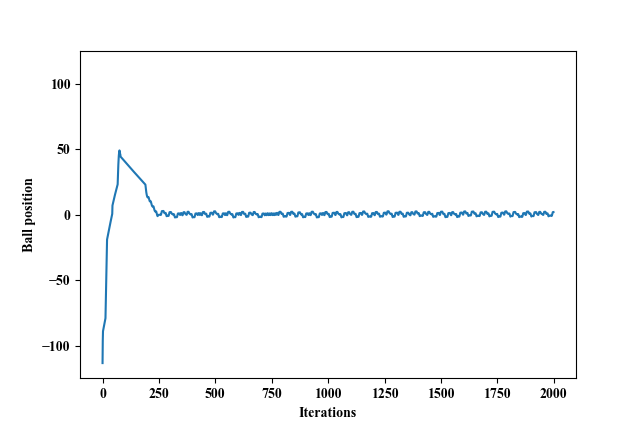
\includegraphics{86_nn}
	\caption{The position of the ball in simulation or 2000 time steps for the trained neural network. The ball starts at the side and is moved closer to the center. It overshoots the centre at first but is moved back and stays in the middle for the remainder of the time.}
	\label{nn_param_test}
\end{figure}

\subsection{Specific Reward Q-learning with Robot}
\subsection{General Reward Q-learning with Robot}
Performance was not good with the robot. As seen in figure \ref{q_nao}, the ball hits the sides of the tray numerous times. There are some instances of getting the ball under control when it is in the middle of the tray, as seen by the changes of direction around the center of the y-axis. Control of the ball is always lost straight away.
\begin{figure}[H]
	\centering
    \subfloat[Instance 1]{{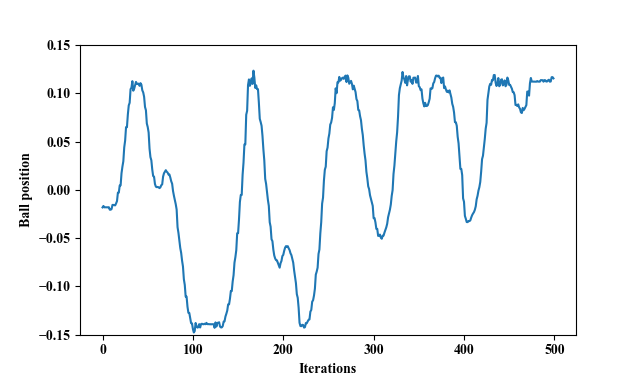
\includegraphics[width=8.5cm]{0_nao_q} }}%
    \subfloat[Instance 2]{{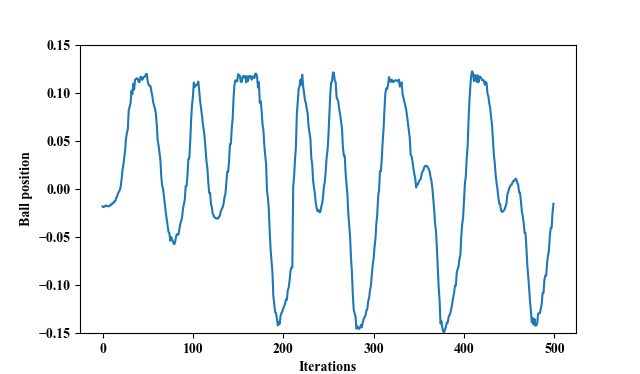
\includegraphics[width=8.5cm]{1_nao_q} }}%
	\caption{Two instances of the ball balancing on the tray with the robot in control. Actions are decided by the trained Q-matrix. Two different cases were shown since performance on the robot could vary quite a lot.}
	\label{q_nao}
\end{figure}
\subsection{Neural Network with Robot}
Performance of the balancing behaviour on the robot was worse than in simulation. The performance was not bad enough to be considered a failure however. Figure \ref{nn_nao} shows the ball position changing over time on the robot. In both cases it does touch the end a few times, but the behaviour does mirror the behaviour in smulation. That is, as the ball approaches the end of the tray, the tray tilts to oppose the movement and the ball rolls in the opposite direction. most of the changes in direction keep the ball away from the sides of the tray. This is evident from the changes of direction in both graphs in figure \ref{nn_nao}.
\begin{figure}[H]
	\centering
    \subfloat[Instance 1]{{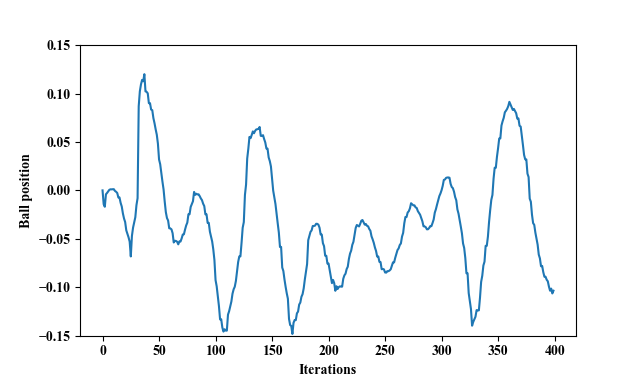
\includegraphics[width=8.5cm]{8_nn_nao} }}%
    \subfloat[Instance 2]{{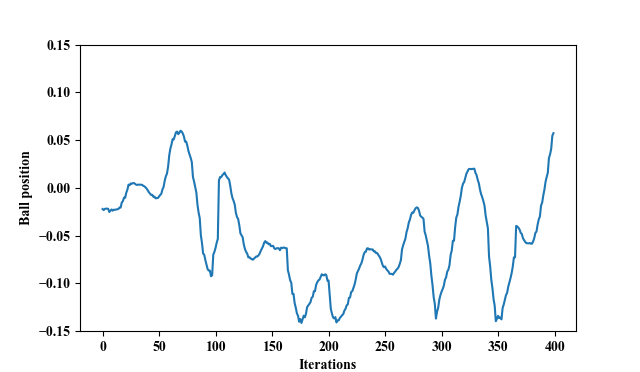
\includegraphics[width=8.5cm]{9_nn_nao} }}%
	\caption{Two instances of the ball balancing on the tray with the robot in control. Actions are decided by the trained neural network. Two different cases were shown since performance on the robot could vary quite a lot.}
	\label{nn_nao}
\end{figure}
\subsection{Refined Q-learning in Simulation}
The first refinement technique to be tested was the inclusion of a delay between actions, and an increase in the speed of the ball in the simulation. The delayed actions help mimic the robot because the robot can take actions less frequently than the simulation. THis is because of the time taken for the robot to execute an action, as well as the frequency of obtaining state information. The increased ball speed in the simulation more accurately represents the speed of the ball in the real world. The original variance in ball speed between robot and simulation could be down to a range of factors including friction between the ball and tray and weight of the ball.

The same parameter refinement as the original simulation was carried out in case the results differed. It was found that most of the best parameters from the original simulation were still the best parameters. The only difference was exploration rate reduction value, where a value of 50\% reduction was found to be marginally better than 33\%, but only by observation of the graphs after the few tests run for each set of parameters. The difference in performance was minimal.

The overall performance of the learnt model was worse with the delay and ball speed up. It did still perform to a level that could be considered balancing, and did not touch the end of the tray very often. Figure \ref{refined_sim_general} shows the behaviour after 50000 iterations. This decrease in performance is not unsurprising since the tray can make adjustments less frequently so has fewer chances to counteract the movement of the ball. The increased speed of the ball also means any movement the ball makes will cover more distance and it will hit the sides quicker.

\begin{figure}[H]
	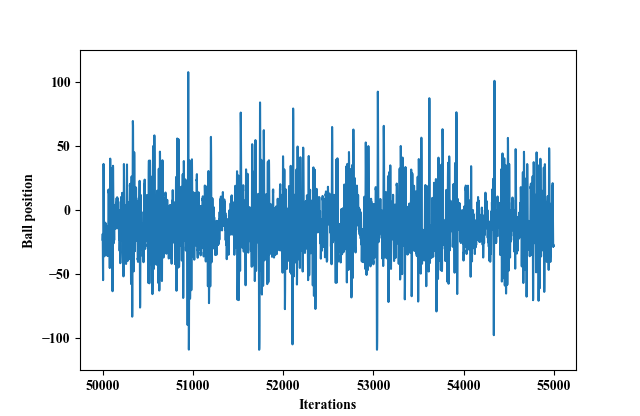
\includegraphics{195}
	\caption{The position of the ball when training with the delay and increased ball speed. The ball rolls to the edges a few times over the 5000 time steps, but the tray gets it under control again. }
	\label{refined_sim_general}
\end{figure}

The next stage of refined learning was experience replay. SAY AMOUNT OF ER DATA

Doing just ER by itself could lead to the ball becoming stuck. THis is due to differnces between the physics of the simulation and the robot. SInce the behaviour is learnt purely from the experiences on the actual robot, the accuracy of the simulation to the robot was irrelevant for training, so this issue only arises when viewing the leanrt behaviour in simulation. When plotting the change of Q-values over time, it can be seen that the values chosen here converge. However, the action that is optimal can change for some pairs of actions. This shows that both actions are essentually equal in their quality. THis means that the one that is considered best can change over time, and the time that the training is stopped determines which is optimal. Since The action with the highest value is outright chosen each time, the other action which is equally as good may not be. Of course in many cases it is not the case that both ations are equally good. in fact in a task like this there is almost always a superior action. In the cases that the wrong action is learnt to be optimal however, it can have a big impact such as the ball getting stuck. As a solution to this, an alternative action selection process was implemented. Instead of picking the action with the highest value, there is a chance of picking either action that is proportional to the values of the actions. For each action, its value as a proportion of the sum of all values is found, and this is the chance that actuion is chosen. This means if two actions have very similar values, then they are equally likely to be chosen. THis is only applied if both actions have positive values or both have negative values. In the case where one action is positive and one is negative, then the choice is clear. Frm running the simulations again using the behaviourr learnt from experienc replay, the performance is better. The ballno longer gets stuck at one side, however the overall performance is poor. THis is most likely due to the randomness that is now in the action selection process. As such, this proportional action selection can be considered a trade-off between optimal performance and average performance - if training goes well such that the close-valued actions end up with the optimal action having the higher value, then the performance will be wore. In the case that the not-optimal behaviour is learnt, then the proportional actin slectin prevents any destructive behaviour. The behaviour seen is not good enough to be considered balancing. The behaviour generally tilts the ball from one end to the other, indicating at some learnt behaviour - enough to get the ball away from the immediate edge - but not enough to keep it centered. 

WHY DO ER QVALS CONVERGE TO VALUES BUT NORMAL SIM QVALS DONT - Think this is because there are quite a few cells that are at 0 since no data exists for those cells. This means the 2nd half of the update function can often be low, which is what keeps the q-val bounded. I THINK WE JUST NEED EVEN MORE ER DATA :/



Simulated behaviour is simlar to nao. 

Show results of performance of just delayed simulation, just experience replay alone and then ER with trained Q mat.
\subsection{Refined Q-learning with Robot}
Includes experience replay
\section{Evaluation}
This approach differs from the reinforcement learning approach because the agent is outright told what is a good action to take in a given state. This is not necessarily bad for machine learning, and works well because the ball balancing task is simple. However, in general it might not be suitable for a more complex task, since it is almost impossible to fully describe exactly how an agent should behave. Another downside to this technique is that it requires generation of training data from human input. This means the agent can only really do as well as the human can. 
This technique is useful because it allows for interpolation between states, which means it deals well with unseen circumstances. The neural network always gives an output no matter what, and assuming it has seen some somewhat similar cases it should give a decent output. In contrast, the Q-matrix may have some blank cells that have never been explored before, meaning there is no way to infer what a good action to take would be. Training time and data size are also an advantage with the neural network. The Q-matrix has to store data for every single state, and since a state is a 3-dimensional vector, the state space grows fast, which means training takes a long time too. The neural network stays the same size however, and whilst its size can vary, it will not be close to the size of the Q-matrix. The training data may be quite large, but once the model is trained it is not required. 
\section{Conclusion}


\bibliography{projectpaper}


\end{document}

Magnus' comments:

Generally feels a bit informally written and wordy (longwinded?). Can you tighten up and clarify the language. 

Abstract: needs doing

Solution: Lots of good information in this sections, but it seems like a long essay, not a structured presentation of how your solution met the aims/deliverables. After specifying the task, perhaps return to an overview of the approaches you will take (and why) so the readers knows where they are while reading the next several subsections. Add more precision, e.g. about the number of division you use to discretise for the Q-matrix, i.e. how big is your Q-matrix, adn about the actual structure of the ANN you used. The description of the ANN is very generic. 


Make the task more precise - what constitutes success? Add a picture of the robot and the tray arrangement, and screen shot of simulation. Discuss how simulation is designed to match real problem. 

Maybe give an example of a (small) Q-matrix or Q-table value update.
Confusing: "The neural network stays the same size however, and whilst its size can vary,…”

Results: 
Parameter optimisation section is good, but again wordy. Could you summarise all results from this section in a small table? It is not clear what range of parameters you considered, only what the ‘best’ outcome was and a couple of specific not-as-good cases where you give a graph.

More to add in results and remaining sections.


Questions
- Past or present tense?
- Do all definitions need a reference (/should they, or can I do own definition like supervised learning in intro?)
- Do I need to even explain neural network?
- Is it suitable to just say these parameters were best, or do need to show comparison data?
- Is results lterally just results, or do I also say "i think this is because..."

To review:
- Doing 2 or 3 actions?

To do:
- Plot changing values of a few q-mat cells over time - see how they change and converge